% -- Encoding UTF-8 without BOM
% -- XeLaTeX => PDF (BIBER)

\documentclass{cv-style}     % Add 'print' as an option into the square bracket to remove colours from this template for printing.

\setdefaultlanguage[variant=british]{english}
\sethyphenation[variant=british]{english}{} % Add words between the {} to avoid them to be cut

%----------------------------------------------------------------------------------------
%	Page layout
%----------------------------------------------------------------------------------------
\cvheadheight{3.5cm}
\cvasidewidth{4.7}
\cvasidevpos{3.5}
\cvmainwidth{11.5cm}
\geometry{left=6.4cm, top=2.5cm, right=1cm, bottom=5mm}

%----------------------------------------------------------------------------------------
%	Bibliography
%----------------------------------------------------------------------------------------
\usepackage[sectcntreset]{bibtopic}
\usepackage{natbib}
\bibliographystyle{bib/achemso_perso}
\AtBeginDocument{\nocite{achemso-control}}
%\setlength{\bibsep}{2pt plus 0.3ex}

%----------------------------------------------------------------------------------------
%	hyperlink setup
%----------------------------------------------------------------------------------------
\hypersetup{
    pdftitle=Resume \textbar{} Laura Gomez,%
    pdfauthor=Laura Gomez
}

%----------------------------------------------------------------------------------------
%	Setup las updated text
%----------------------------------------------------------------------------------------
%\lastupdated{Last Updated on \today}

%----------------------------------------------------------------------------------------
%	Add a few custom packages
%----------------------------------------------------------------------------------------
\usepackage{fontawesome5}

% \usepackage{academicons}
% \definecolor{orcidlogocol}{HTML}{A6CE39}

\begin{document}

\header{Laura }{Gomez}{Tecnical Project Manager in Mechatronics and Biomechanics}          % Your name

%----------------------------------------------------------------------------------------
%	SIDEBAR SECTION  -- In the aside, each new line forces a line break
%----------------------------------------------------------------------------------------

\begin{aside}
    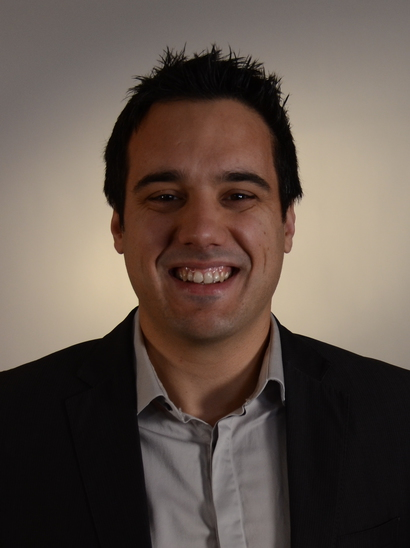
\includegraphics[width=.8\columnwidth]{img/gvallver-red2}
    Immediate availability
    Permis B
    ~
    Nationalité Française
    13 janvier 1989, France
    En concubinage
    %
    \section{Contact}
    laura-gomez@gmx.fr
    +33 7 70 49 23 44
    ~
    91 rue du Colonel Fabien
    92160 Antony
    France
    %
    \section{Contact}
    germain.vallverdu@univ-pau.fr
    (33) 5 59 40 78 51
    (33) 6 88 59 08 87
    ~
    {\color{gray} \faFlask} IPREM
    Technopôle Hélioparc
    2 ave du Président P. Angot
    FR-64053 Pau cedex 9
    \href{http://iprem.univ-pau.fr/fr/index.html}{http://iprem.univ-pau.fr}
    %
    \section{Theoretical Chemistry}
    Computational strategy
    Development
    Complex matrices
    Surfaces, interfaces
    VASP, CRYSTAL (solid)
    Gaussian, Orca (molecule)
    Gromacs, Lammps (MD)
    %
    \section{Programming}
    {\color{gray}\faPython} Python
    Fortran, C
    \LaTeX{}, HTML/CSS
    %
    \section{Languages}
    French
    English 
    %
    \section{Bibliometry}
    18 articles
    13 conferences
    h-\textit{index}: 8
    12.5 citations per item
    199 citations (181 w/o self-citations)
    %
    \section{On the web}
    \href{https://publons.com/researcher/2764008/}{\color{gray}\faNewspaper\small ~publons 2764008}
    %\href{http://orcid.org/0000-0003-1116-8776}{$\vcenter{\hbox{
\includegraphics[height=4mm]{img/orcid_128x128}}}$\small ~orcid.org/0000-0003-1116-8776}
    %\href{https://github.com/gVallverdu}{$\vcenter{\hbox{
\includegraphics[height=16pt]{img/GitHub-Mark}}}$ gVallverdu}
    \href{https://github.com/gVallverdu}{\color{gray}\faGithub\small ~GitHub} \href{https://gitlab.com/gvallverdu}{\color{gray}\faGitlab\small ~GitLab}: {\small gvallverdu} 
    \href{https://gsalvatovallverdu.gitlab.io/}{\color{gray}\faFile*[regular]\small ~gsalvatovallverdu.gitlab.io}
    %
\end{aside}

\vspace{0mm}
\section{Abs}{tract}
\vspace{-0.2cm}


Associate professor at the University of Pau \& Pays Adour, I am a specialist in
theoretical chemistry, molecular modeling and numerical simulations at IPREM institute.
My research activities, in physical-chemistry, concern the understanding 
of macroscopic phenomena such as reactivity, thermochemistry or spectroscopy from
a microscopic description of matter. The implementation and combination of relevant computational
strategies allows for the investigation of complex systems in various field among
petroleum-chemistry, biological systems or energy storage materials.


%Associate professor at the University of Pau \& Pays Adour, I am a specialist in
%theoretical chemistry and numerical simulations at IPREM institute.
%My research activities concern the development of new methods and
%computational strategies at different time or space scales, applied to the
%investigations of complex systems (surfaces, interfaces, complex matrices in
%condensed matter). I teach mainly chemical-physics subjects and programming
%languages at the university of Pau.

% Associate professor at the Université de Pau et des Pays de l'Adour,
% I am a theoretical chemist at IPREM institute (Institute for Analytical sciences and
% chemical physics applied to environment and materials).
% My research activities concern the development of new methods in theoretical chemistry
% and new computational
% strategies at different time or space scales, applied to the investigations
% of complex systems.
% I teach mainly chemical-physics subjects and programming languages at the university of Pau.

%----------------------------------------------------------------------------------------
%	SKILLS SECTION
%----------------------------------------------------------------------------------------

%\section{skills}
%  \vspace{-0.2cm}

%Skill 1, skill 2, skill 3, skill 4, skill 5.

%----------------------------------------------------------------------------------------
%	WORK EXPERIENCE SECTION
%----------------------------------------------------------------------------------------
\vspace{-2mm}
\section{Professional }{Experiences}
\vspace{-0.3cm}

\begin{entrylist}
%------------------------------------------------
\entry
  {since 2010~}
  {Université de Pau et des Pays de l'Adour}
  {Pau, France}
  {\jobtitle{Associate professor}\\
   Theoretical chemistry and computational approaches.
   Surfaces, interfaces, reactivity and molecular interactions.}
%------------------------------------------------
\entry
  {2009--2010}
  {CEA - DAM}
  {Bruyères le châtel, France}
  {
  \jobtitle{Postdoctoral position}\\
  Development and implementation of a mesoscopic model for reactive shock waves
  propagation in heterogeneous systems.
  }
%------------------------------------------------
\entry
  {2006--2009}
  {Université Paris-Sud 11}
  {Orsay, France}
  {
  \jobtitle{PhD Student}\\
  Theoretical study of photophysical processes in fluorescent proteins.
  }
%------------------------------------------------
\end{entrylist}

%----------------------------------------------------------------------------------------
%	EDUCATION SECTION
%----------------------------------------------------------------------------------------
\vspace{-5mm}
\section{Educ}{ation}
\vspace{-0.2cm}

\begin{entrylist}
%------------------------------------------------
\entry
{2006-2009}
{PhD in chemistry {\normalfont speciality theoretical chemistry}}
{Université Paris-Sud 11}
{Mention très honorable}
%------------------------------------------------
\entry
{2004-2006}
{Master degree of physical-chemistry}
{Université Paris-Sud 11}
{{\normalfont speciality \textit{Physico-Chimie Moléculaire}}\par Mention TB}
%------------------------------------------------
\entry
{2003-2004}
{Bachelor Degree of physical-chemistry}
{Université Paris-Sud 11}
{Mention TB}
%------------------------------------------------
\entry
{2003-2006}
{Magistère de Physico-Chimie Moléculaire}
{Université Paris-Sud 11 -- ENS Cachan}
{\vspace{-4mm}}
%------------------------------------------------
\entry
{2001-2003}
{Undergraduate {\normalfont physics and chemistry}}
{Lycée François Arago, Perpignan}
{}
\end{entrylist}

%----------------------------------------------------------------------------------------
%	OTHER QUALIFICATIONS SECTION
%----------------------------------------------------------------------------------------
\vspace{-6mm}
\section{Main}{ publications}
\vspace{-0.2cm}
\nocite{munoz2019, santos2018, aqturin2017_2, santos2017, vallverdu2016, Maillet2011, Vallverdu2010}
%\nocite{santos2018, aqturin2017_2, santos2017, vallverdu2016, Martin2012, Maillet2011, Vallverdu2010}
\begin{btSect}{bib/cv_articles}
    \setlength{\bibsep}{2pt}
    \btPrintCited
\end{btSect}

%----------------------------------------------------------------------------------------
%	INTERESTS SECTION
%----------------------------------------------------------------------------------------

% \section{interests}
%   \vspace{-0.2cm}
%
% \textbf{professional:} professional interest 1, professional interest 2 and professional interest 3.
% \textbf{personal:} personal interest 1, personal interest 2, personal interest 3 and personal interest 4.

%----------------------------------------------------------------------------------------
%	TEACHING SECTION
%----------------------------------------------------------------------------------------
\vspace{-1mm}
\section{Teach}{ing}
  \vspace{-0.3cm}

$\bullet$ Lectures in chemical-physics, theoretical chemistry and programming languages.\\
%in bachelor degrees, master degrees and doctoral school. About 200 h/year\\
$\bullet$ Strong involvement in new information and communication technologies for education\\
$\bullet$ Science popularization: Quantum mechanics and workshops for school students
%organization of animations for secondary and primary school pupils.

\vspace*{-5mm}

%\begin{itemize}
%    \item Lectures in chemical-physics, theoretical chemistry and programming languages, in bachelor
%    degrees, master degrees and doctoral school.
%    \item Science popularization: Quantum mechanics, animations for secondary and primary school pupils
%\end{itemize}

%----------------------------------------------------------------------------------------

\end{document}
